%%%%%%%%%%%%%%%%%%%%%% file template.tex %%%%%%%%%%%%%%%%%%%%%%%%%
%
% This is a general template file for the LaTeX package SVJour3
% for Springer journals.          Springer Heidelberg 2010/09/16
%
% Copy it to a new file with a new name and use it as the basis
% for your article. Delete % signs as needed.
%
% This template includes a few options for different layouts and
% content for various journals. Please consult a previous issue of
% your journal as needed.
%
%%%%%%%%%%%%%%%%%%%%%%%%%%%%%%%%%%%%%%%%%%%%%%%%%%%%%%%%%%%%%%%%%%%

\RequirePackage{fix-cm}

%\documentclass{svjour3}                     % onecolumn (standard format)
%\documentclass[smallcondensed]{svjour3}     % onecolumn (ditto)
\documentclass[smallextended]{svjour3}       % onecolumn (second format)
%\documentclass[twocolumn]{svjour3}          % twocolumn

\smartqed  % flush right qed marks, e.g. at end of proof

% \usepackage[small,bf]{caption}
% \usepackage{titlesec}
% \titleformat{\section}{\large\bfseries}{\thesection}{1em}{}
\usepackage{graphicx}
\usepackage{amsfonts}
\usepackage{amssymb}
\usepackage{amsmath}
\usepackage[table]{xcolor}
\definecolor{lightgray}{gray}{0.9}
% \usepackage{german}
% \usepackage{hebtex}
% \usepackage[german]{babel}
% \usepackage{endnotes}
% \let\footnote=\endnote
% \usepackage{rotating}
\usepackage{enumerate}

% please place your own definitions here and don't use \def but
% \newcommand{}{}
%
\newcommand{\nias}{\noindent} % no indent after new section
\newcommand{\nial}{\noindent} % no indent after equation, list, or whatever
\newcommand{\nonsc}[1]{}
\newcommand{\qnull}[1]{`#1'}
\newcommand{\qeins}[1]{``#1''}
\newcommand{\qzwei}[1]{`#1'}
\newcommand{\erf}[0]{\mbox{erf}}
\newcommand{\anum}[0]{a'}
\newcommand{\bnum}[0]{b'}
\newcommand{\cnum}[0]{c'}
\newcommand{\hnum}[0]{h'}
\newcommand{\knum}[0]{k'}
\newcommand{\wnum}[0]{w'}
\newcommand{\aden}[0]{a''}
\newcommand{\bden}[0]{b''}
\newcommand{\cden}[0]{c''}
\newcommand{\hden}[0]{h''}
\newcommand{\kden}[0]{k''}
\newcommand{\wden}[0]{w''}
\newcommand{\lwv}[0]{0.6}
\newcommand{\qvu}[0]{\vartheta}
% \newif\ifNumericalOrYear
% \NumericalOrYeartrue
% \NumericalOrYearfalse
% \ifNumericalOrYear
% \usepackage[numbers,colon]{natbib}
% \else
% \usepackage[round,colon]{natbib}
% \usepackage{natbib}
% \fi
\newif\ifPageP
\PagePtrue
\PagePfalse
\ifPageP
\newcommand{\PageP}{p.~}
\else
\newcommand{\PageP}{}
\fi
% \newcommand{\scite}[3]{\ifnum#1=1\ifNumericalOrYear\citep{#2}\else\citeyearpar{#2}\fi\else
% \ifnum#1=2\ifNumericalOrYear\citep[#3]{#2}\else\citep[{\PageP}#3]{#2}\fi\else
% \ifnum#1=3\ifNumericalOrYear(\citet[#3]{#2})\else\citep[{\PageP}#3]{#2}\fi\else
% \ifnum#1=4\ifNumericalOrYear\citet{#2}\else\citet{#2}\fi\else
% \ifnum#1=5\ifNumericalOrYear(\citet{#2})\else\citep{#2}\fi\else
% \ifnum#1=6\ifNumericalOrYear(\citet[#3]{#2})\else\citep[{\PageP}#3]{#2}\fi\else
% \ifnum#1=7\ifNumericalOrYear\citep{#2}\else\citealp{#2}\fi\else
% \ifnum#1=8\ifNumericalOrYear\citep[#3]{#2}\else\citealp[{\PageP}#3]{#2}\fi\else
% \ifnum#1=9\ifNumericalOrYear\citep[#3]{#2}\else{}loc.\ cit., {\PageP}#3\fi\else
% \textbf{[invalid scite code]}\fi\fi\fi\fi\fi\fi\fi\fi\fi}
\newcommand{\scite}[3]{\ifnum#1=1\cite{#2}\else
\ifnum#1=2\cite[{\PageP}~#3]{#2}\else
\ifnum#1=3\cite[{\PageP}~#3]{#2}\else
\ifnum#1=4\cite{#2}\else
\ifnum#1=5\cite{#2}\else
\ifnum#1=6\cite[{\PageP}~#3]{#2}\else
\ifnum#1=7\cite{#2}\else
\ifnum#1=8\cite[{\PageP}~#3]{#2}\else
\ifnum#1=9\cite[{\PageP}~#3]{#2}\else
\textbf{[invalid scite code]}\fi\fi\fi\fi\fi\fi\fi\fi\fi}
% \newcommand{\scite}[3]{#2}
% \newcommand{\scite}[3]{\cite{#2}}

\newenvironment{quotex}{\begin{quote}\begin{footnotesize}}{\end{footnotesize}\end{quote}}

% Insert the name of "your journal" with
\journalname{Synthese}

\begin{document}

\title{The Principle of Maximum Entropy and a Problem in Probability Kinematics}
% \subtitle{Do you have a subtitle?\\ If so, write it here}

\author{Stefan Lukits}

\institute{Stefan Lukits \at
University of British Columbia \\
Department of Philosophy \\
1866 Main Mall E370 \\
Vancouver BC Canada V6T 1Z1 \\
\email{saiserit@streetgreek.com}
}
% \institute{for blind review}

\date{Received: date / Accepted: date}
% The correct dates will be entered by the editor

\maketitle

\begin{abstract}
  \noindent Given a more general type of evidence than Bayes' formula
  will accommodate, the principle of maximum entropy (\textsc{maxent})
  provides a unique solution for the posterior probability
  distribution based on the intuition that the information gain
  consistent with assumptions and evidence should be minimal.
  Opponents of objective methods to determine these probabilities
  prominently cite van Fraassen's Judy Benjamin case to undermine the
  generality of \textsc{maxent}. This article shows that an intuitive
  approach to Judy Benjamin's case supports \textsc{maxent}. This is
  surprising because based on independence assumptions the anticipated
  result is that it would support the opponents. It also demonstrates
  that opponents improperly apply independence assumptions to the
  problem.
  \keywords{Judy Benjamin \and Principle of Maximum Entropy \and
    Coarsening at Random \and Full Employment Theorem \and Probability
    Kinematics \and Epistemic Entrenchment}
\end{abstract}

\section{Introduction}
\label{Introduction}

Probability kinematics is the field of inquiry asking how we should
update a probability distribution in the light of evidence. If the
evidence comes as an event, it is relatively uncontroversial to use
conditional probabilities (call this standard conditioning).
Sometimes, however, the evidence may not relate the certainty of an
event but a reassessment of its uncertainty or its probabilistic
relation to other events (see \scite{8}{jeffrey65}{153ff}),
expressible in a shift in expectation (see \scite{7}{hobson71}{}).
Jeffrey conditionalization can deal with some of these cases, but not
with all of them (see figure~\ref{fig:aff}). Bas van Fraassen has come
up with an example for a case in which we cannot apply Jeffrey
conditionalization. The example is from the 1980 comedy film
\emph{Private Benjamin} (see \scite{7}{fraassen81}{})\nonsc{}, in
which Goldie Hawn portrays a Jewish-American woman (Judy Benjamin) who
joins the U.S. Army.

\begin{figure}[h!]
  \begin{flushright}
    \begin{minipage}[h]{.8\linewidth}
      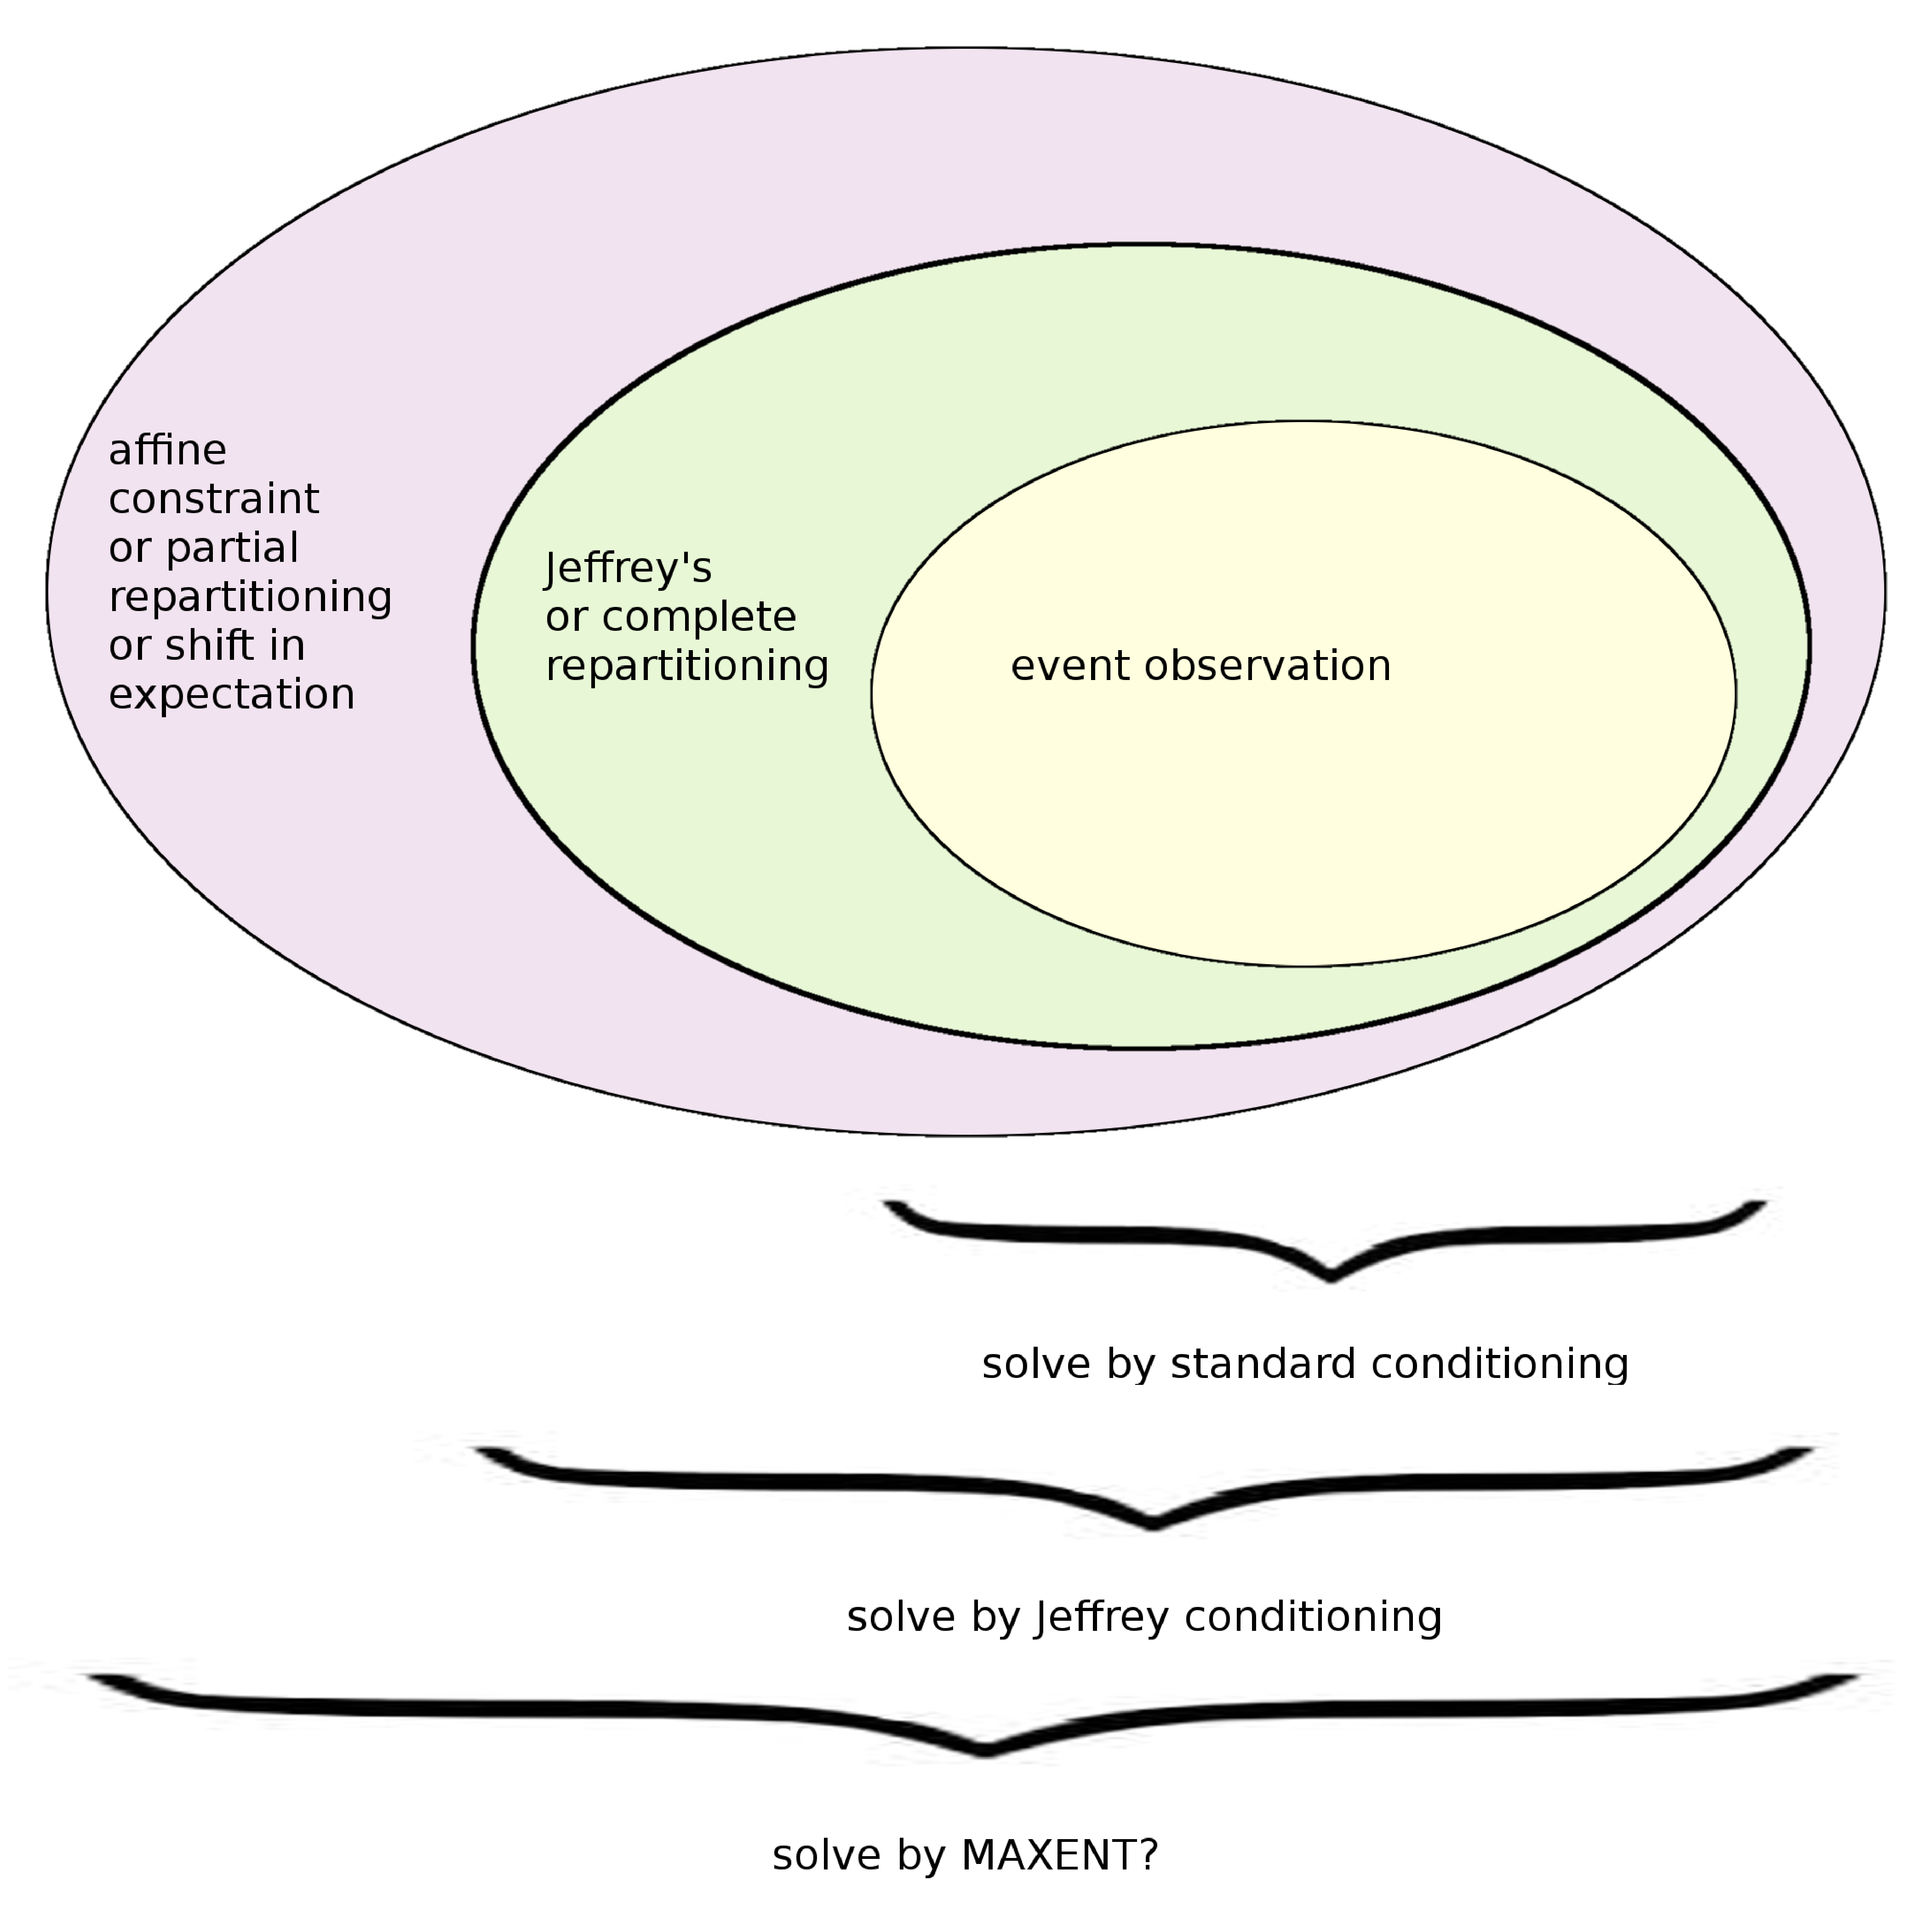
\includegraphics[width=\textwidth]{affine1.eps}
      \caption{Information that leads to unique solutions for
        probability updating using \textsc{maxent} must come in the
        form of an affine constraint (a constraint in the form of an
        informationally closed and convex space of probability
        distributions consistent with the information). All
        information that can be processed by Jeffrey conditioning
        comes in the form of an affine constraint, and all information
        that can be processed by standard conditioning can also be
        processed by Jeffrey conditioning. The solutions of
        \textsc{maxent} are consistent with the solutions of Jeffrey
        conditioning and standard conditioning where the latter two
        are applicable.}
      \label{fig:aff}
    \end{minipage}
  \end{flushright}
\end{figure}

\begin{figure}[h!]
  \begin{flushright}
    \begin{minipage}[h]{.8\linewidth}
      \includegraphics[width=\textwidth]{judy.eps}
      \caption{Judy Benjamin's map. Blue territory ($A_{3}$) is friendly and
        does not need to be divided into a Headquarters and a Second
        Company area.}
      \label{fig:map}
    \end{minipage}
  \end{flushright}
\end{figure}

In van Fraassen's interpretation of the movie, Judy Benjamin is on an
assignment and lands in a place where she is not sure of her location.
She is on team Blue. Because of the map, initially the probability of
being in Blue territory equals the probability of being in Red
territory, and the probability of being in the Red Second Company area
equals the probability of being in the Red Headquarters area. Her
commanders then inform Judy by radio that in case she is in Red
territory, her chance of being in the Red Headquarters area is three
times the chance of being in the Red Second Company area. The question
is what Judy's appropriate response is to this new evidence.

We cannot apply standard conditioning, because there is no immediately
obvious event space in which we can condition on an event of which we
are certain. Grove and Halpern \scite{1}{grovehalpern97}{} have
offered a proposal for constructing such event spaces and then
conditioning on the event that Judy Benjamin receives the information
that she receives from her commanders. They admit, however, that the
construction of such spaces (sometimes called retrospective
conditioning) is an exercise in filling in missing details and
supplying information not contained in the original problem.

If we assume that the attempt fails to define an event on which Judy
Benjamin could condition her probabilities, we are left with two
possibilities. Her new information (it is three times as likely to
land in $A_{2}$ than to land in $A_{1}$, see figure~\ref{fig:map} and
the details of the problem in the next section) may mean that we have
a redistribution of a complete partition of the probabilities. This is
called Jeffrey conditioning and calls for Jeffrey's rule. Jeffrey's
rule is contested in some circles, but we will for this project accept
its validity in probability kinematics. We will see in what follows
that some make the case that Jeffrey conditioning is the correct way
to solve the Judy Benjamin problem. For reasons provided in the body
of the paper their case is implausible.

The third possibility to solve this problem (after standard
conditioning and Jeffrey conditioning) is to consult a highly
contested updating procedure: the principle of maximum entropy
(\textsc{maxent} for short). \textsc{maxent} can be applied to any
situation in which we have a completely quantified probability
distribution and an affine constraint (we will explain the nature of
affine constraints in more detail later). If our new evidence is the
observation of an event (or simply certainty about an event that we
did not have previously), then the event provides an affine constraint
and can be used for updating by means of standard conditioning. If our
new evidence is a redistribution of probabilities where we can apply
Jeffrey's rule, then the redistribution provides an affine constraint
and can be used for updating by means of Jeffrey's rule. These two
possibilities, however, do not exhaust affine constraints. The Judy
Benjamin problem illustrates the third possibility where the affine
constraint only redistributes some groups of probabilities and leaves
open the question how this will affect the probabilities not included
in this redistribution.

Advocates of \textsc{maxent} claim that in this case the probabilities
should be adjusted so that they are minimally affected (we make this
precise by using information theory) while at the same time according
with the constraint. Opponents of this view grant that \textsc{maxent}
is an important tool of probability kinematics. Noting that some
results of \textsc{maxent} are difficult to accept (such as in the
Judy Benjamin case), however, they urge us to embrace a more
pluralistic, situation-specific methodology.

Joseph Halpern, for example, writes in \emph{Reasoning About
  Uncertainty} that \qeins{there is no escaping the need to understand
  the details of the application} \scite{2}{halpern03}{423} and
concludes that \textsc{maxent} is a valuable tool, but should be used
with care (see \scite{8}{grovehalpern97}{110}), explicitly basing his
remark on the counterintuitive behaviour of the Judy Benjamin problem.
Diaconis and Zabell state \qeins{that any claims to the effect that
  maximum-entropy revision is the only correct route to probability
  revision should be viewed with considerable caution}
\scite{2}{diaconiszabell82}{829}. \qeins{Great caution} (1994,
456)\nonsc{} is also what Colin Howson and Allan Franklin advise about
the more basic claim that the updated probabilities provided by
\textsc{maxent} are as like the original probabilities as it is
possible to be given the constraints imposed by the data.

In the same vein, Igor Douven and Jan-Willem Romeijn agree with
Richard Bradley that \qeins{even Bayes' rule \qzwei{should not be
    thought of as a universal and mechanical rule of updating, but as
    a technique to be applied in the right circumstances, as a tool in
    what Jeffrey terms \emph{the art of judgment}.} In the same way,
  determining and adapting the weights {\ldots} may be an art, or a
  skill, rather than a matter of calculation or derivation from more
  fundamental epistemic principles} \scite{2}{douvenromeijn09}{16}
(for the Bradley quote see \scite{8}{bradley05}{362}).

What is lacking in the literature is a response by \textsc{maxent}
advocates to the counterintuitive behaviour of the cases repeatedly
quoted by their adversaries. This is especially surprising as we are
not dealing with an array of counter-examples but only a handful, the
Judy Benjamin problem being prime among them. In Halpern's textbook,
for example, the reasoning is as follows: \textsc{maxent} is a
promising candidate which delivers unique updated probability
distributions; but, unfortunately, there is counterintuitive behaviour
in one specific case, the Judy Benjamin case (see
\scite{8}{halpern03}{110, 119}); therefore, we must abide by the
eclectic principle of considering not only \textsc{maxent}, but also
lower and upper probabilities, Dempster-Shafer belief functions,
possibility measures, ranking functions, relative likelihoods, and so
forth. The human inquirer is the final arbiter between these
conditionalization methods.

At the heart of our investigation are two incompatible but
independently plausible intuitions regarding Judy's choice of updated
probabilities for her location. We will undermine the notion that
\textsc{maxent}'s solution for the Judy Benjamin problem is
counterintuitive. The intuition that \textsc{maxent}'s solution for
the Judy Benjamin problem violates (call it T1) is based on fallacious
independence and uniformity assumptions. There is another powerful
intuition (call it T2) that conflicts with T1 and obeys
\textsc{maxent}. Therefore, Halpern does not give us sufficient
grounds for the eclecticism advocated throughout his book. We will
show that another intuitive approach, the powerset approach, lends
significant support to the solution provided by \textsc{maxent} for
the Judy Benjamin problem, especially in comparison to intuition T1,
many of whose independence and uniformity assumptions it shares. 

We have no proof that \textsc{maxent} is the only rationally
defensible objective method to update probabilities given an affine
constraint. The literature outlines many of the \qnull{nice
  properties} of \textsc{maxent}. It seamlessly generalizes standard
conditioning and Jeffrey's rule where they are applicable (see
\scite{7}{catichagiffin06}{}). It underlies the entropy concentration
phenomenon described in Jaynes' standard work \emph{Probability
  Theory: the Logic of Science}, which contains other arguments in
favour of \textsc{maxent} (some of which you may recognize by family
resemblance in the rest of this paper). Entropy concentration refers
to the unique property of the \textsc{maxent} solution to have other
distributions which obey the affine constraint cluster around it.
Shore and Johnston have shown that under certain rationality
assumptions \textsc{maxent} provides the unique solution to problems
of probability updating (see \scite{7}{shorejohnson80}{}). When used
to make predictions whose quality is measured by a logarithmic score
functions, posterior probabilities provided by \textsc{maxent} result
in minimax optimal decisions (see \scite{7}{topsoe79}{},
\scite{7}{walley91}{}, and \scite{7}{grunwald00a}{}). Under a
logarithmic scoring rule these posterior probabilities are in some
sense optimal.

Despite all these nice properties, we want the reader to follow us in
a more simple line of argument. When new evidence is provided to us,
it is rational to adjust our beliefs minimally in light of it. We do
not want to draw out more information from the new evidence than
necessary. We are the first to admit that there are numerous problems
here that need addressing. What do we mean by rationality? What are
the semantics of the word \qnull{minimal}? What are the formal
properties of such posterior probabilities? Are they unique? Are they
compatible with other intuitive methods of updating? Are there
counter-intuitive examples that would encourage us to give up on this
line of thought rather than live with its consequences? Given some
decent answers to these questions, however, we feel that
\textsc{maxent} cuts a good figure as a first pass to provide
objective solutions to these types of problems, and the burden on
opponents who usually deny that there are such objective solutions
exist grows heavy.

The distinctive contribution of this paper is to show why the
reasoning of the opponents of \textsc{maxent} in the Judy Benjamin
case is flawed. They make independence assumptions that on closer
inspection do not hold up. We provide a number of scenarios consistent
with the information in the problem which violate these independence
assumptions. That does not mean that the information given in the
problem suggests these scenarios, it only means that we are not
entitled to make those independence assumptions. That, in turn, does
not privilege the \textsc{maxent} solution, although \textsc{maxent}
does not lean on independence assumptions that other solutions
illegitimately make. \textsc{maxent}, however, confronts us with a
much stronger claim than merely providing a passable or useful
solution to the Judy Benjamin problem: it claims to much greater
generality and, to use a term abjured by many formal epistemologists,
to objectivity. These claims must be motivated elsewhere, and the
nature of their normativity is a matter of debate (for a pragmatic
approach see \scite{7}{caticha12}{}). We are only showing that
opponents cannot claim an easy victory by pulling out old Judy
Benjamin.

There is a long-standing disagreement between (mostly) philosophers on
the one hand and (mostly) physicists on the other hand. The
philosophers claim that updating probabilities is irreducibly
accompanied by thoughtful deliberation with the choice between
different updating procedures depending on individual problems. The
physicists claim that problems are ill-posed if they do not contain
the information necessary to let a non-arbitrary, objective procedure
(such as \textsc{maxent}) arrive at a unique updated probability
distribution. In the literature, Judy Benjamin serves as an example
widely taken to count in favour of the philosophers. It is taken to
support what I shall call the full employment theorem of probability
kinematics.

The full employment theorem of probability kinematics claims that
\textsc{maxent} is only one of many different strategies to update
probabilities. In order to decide which strategy is the most
appropriate for your problem you need a resident formal epistemologist
to do the thinking and weigh the intuitions for you. For a fee, of
course. Thus formal epistemologists will always be fully employed.
(E.T. Jaynes makes similar observations when he derisively talks about
the statistician-client relationship as one between a doctor and his
patient, see \scite{8}{jaynes98}{492 and 506}.) There is an analogous
full employment theory in computer science about writing computer
programs which has been formally proven to be true. Our contention is
that no such proof is forthcoming in probability kinematics. 

\section{Two Intuitions}
\label{TwoIntuitions}

There are two pieces of information relevant to Judy Benjamin
when she decides on her updated probability assignment. We will call
them ({\ref{eq:map}}) and ({\ref{eq:hdq}}). As in
figure~\ref{fig:map}, $A_{1}$ is the Red Second Company area, $A_{2}$ is
the Red Headquarters area, $A_{3}$ is Blue territory. Judy presumably
wants to be in Blue territory, but if she is in Red territory, she
would prefer their Second Company area (where enemy soldiers are not
as well-trained as in the Headquarters area).

\begin{enumerate}
\item[({\ref{eq:map}})] Judy has no idea where she is. Because of the
  map, her probability of being in Blue territory equals the
  probability of being in Red territory, and the probability of being
  in the Red Second Company area equals the probability of being in
  the Red Headquarters area.
\item[({\ref{eq:hdq}})] Her commanders inform Judy that in case she is in Red
  territory, her chance of being in their Headquarters area is three
  times the chance of being in their Second Company area.
\end{enumerate}

\nial In formal terms (sloppily writing $A_{i}$ for the event of Judy
being in $A_{i}$),

\begin{equation}
  \label{eq:map}
  2\cdot{}P(A_{1})=2\cdot{}P(A_{2})=P(A_{3})\tag{\mbox{MAP}}
\end{equation}
\begin{equation}
  \label{eq:hdq}
  {\qvu}=P(A_{2}|A_{1}\cup{}A_{2})=\frac{3}{4}\tag{\mbox{HDQ}}
\end{equation}

\nial ({\ref{eq:hdq}}) is partial information because in contrast to
the kind of evidence we are used to in Bayes' formula (such as
\qnull{an even number was rolled}), and to the kind of evidence needed
for Jeffrey's rule (where a partition of the whole event space and its
probability redistribution is required, not only $A_{1}\cup{}A_{2}$,
but see here the objections in \scite{7}{douvenromeijn09}{}), the
scenario suggests that Bayesian conditionalization and Jeffrey's rule
are inapplicable. We are interested in the most defensible updated
probability assignment(s) and will express them in the form of a
normalized odds vector $(q_{1},q_{2},q_{3})$, following van Fraassen
\scite{1}{fraassen81}{}. $q_{i}$ is the updated probability $Q(A_{i})$
that Judy Benjamin is in $A_{i}$. Let $P$ be the probability
distribution prior to the new observation and $p_{i}$ the individual
\qnull{prior} probabilities. These probabilities are not to be
confused with prior probabilities that precede any kind of
information. In the spirit of probability update, or probability
kinematics, we will for the rest of the article refer to prior
probabilities as probabilities prior to an observation and the
subsequent update. The $q_{i}$ sum to $1$ (this differs from van
Fraassen's canonical odds vector, which is proportional to the
normalized odds vector but has $1$ as its first element). We define
\begin{displaymath}
  t=\frac{{\qvu}}{1-{\qvu}}
\end{displaymath}

\nial $t$ is the factor by which ({\ref{eq:hdq}}) indicates that
Judy's chance of being in $A_{2}$ is greater than being in $A_{1}$. In
Judy's particular case, $t=3$ and ${\qvu}=0.75$. Two intuitions guide
the way people think about Judy Benjamin's situation.

\begin{enumerate}
  \item[\textbf{T1}] ({\ref{eq:hdq}}) does not refer to Blue territory and
  should not affect $P(A_{3})$: $q_{3}=p_{3}(=0.50)$.
\end{enumerate}

\nial There is another, conflicting intuition (due to Peter Williams
via personal communication with van Fraassen, see
\scite{8}{fraassen81}{379})\nonsc{}:

\begin{enumerate}
\item[\textbf{T2}] If the value of ${\qvu}$ approaches $1$ (in other words,
  $t$ approaches infinity) then $q_{3}$ should approach $2/3$ as the
  problem reduces to one of ordinary conditioning. ({\ref{eq:hdq}})
  would turn into \qnull{if you are in Red territory you are almost
    certainly in the Red Headquarters area.} Considering
  ({\ref{eq:map}}), $q_{3}$ should approach $2/3$. 
\end{enumerate}

\nial Continuity considerations pose a contradiction to T1. (These
considerations are strong enough that Luc Bovens uses them as an
assumption to solve Adam Elga's Sleeping Beauty problem by parity of
reasoning in \scite{7}{bovens10}{}.) To parse these conflicting
intuitions, we will introduce several methods to provide $G$, the
function that maps ${\qvu}$ to the appropriate normalized updated odds
vector $(q_{1},q_{2},q_{3})$. 

The first method is extremely simple and accords with intuition T1:
$G_{\mbox{{\tiny ind}}}({\qvu})=(0.5(1-{\qvu}),0.5{\qvu},0.5)$. In
Judy's particular case with $t=3$ the normalized odds vector is (ind
stands for independent):
\begin{displaymath}
  G_{\mbox{{\tiny ind}}}(0.75)=(0.125,0.375,0.500)
\end{displaymath}

\nial Both Grove and Halpern \scite{1}{grovehalpern97}{} and Douven
and Romeijn \scite{1}{douvenromeijn09}{} make a case for this
distribution. Grove and Halpern use standard conditioning on the event
of the message being transmitted to Judy. Douven and Romeijn use
Jeffrey's rule (because they believe that T1 is in this case so strong
that $Q(A_{3})=P(A_{3})$ is as much of a constraint as (\ref{eq:map})
and (\ref{eq:hdq}), yielding a Jeffrey partition). 

T1, however, conflicts with the symmetry requirements outlined in van
Fraassen et.\ al.\ \scite{1}{fraassenetal86}{}. Van Fraassen
introduces various updating methods which do not conflict with those
symmetry requirements, the most notable of which is \textsc{maxent}.
Shore and Johnson have already shown that, given certain assumptions
(which have been heavily criticized, e.g.\ in \scite{7}{uffink96}{}),
\textsc{maxent} produces the unique updated probability assignment
according with these assumptions. The minimum information
discrimination theorem of Kullback and Leibler (see for example
\scite{7}{csiszar67}{}, section 3) demonstrates how Shannon's entropy
and the Kullback-Leibler Divergence formula can provide the least
informative updated probability assignment (with reference to the
prior probability assignment) obeying the constraint posed by the
evidence. The idea is to define a space of probability distributions,
make sure that the constraint identifies a closed, convex subset in
this space, and then determine which of the distributions in the
closed, convex subset is least distant from the prior probability
distribution in terms of information (using the minimum information
discrimination theorem). It is necessary for the uniqueness of this
least distant distribution that the subset be closed and convex (in
other words, that the constraint be affine, see
\scite{7}{csiszar67}{}).

For Judy Benjamin, \textsc{maxent} suggests the following normalized
odds vector:
\begin{equation}
  \label{eq:vmax}
  G_{\mbox{{\tiny max}}}(0.75)\approx(0.117,0.350,0.533)
% use testgenq.m for this, see page 143 in Green Book
\end{equation}
The updated probability of being on Blue territory ($A_{3}$) has
increased from 50\% to approximately 53\%. Grove and Halpern find this
result \qeins{highly counterintuitive} \scite{2}{grovehalpern97}{2}.
Van Fraassen summarizes the worry:
\begin{quotex}
  It is hard not to speculate that the dangerous implications of being
  in the enemy's Headquarters area are causing Judy Benjamin to
  indulge in wishful thinking, her indulgence becoming stronger as her
  conditional estimate of the danger increases. \scite{3}{fraassen81}{379}
\end{quotex}

\bigskip

\nial There are two ways in which we can arrive at result
({\ref{eq:vmax}}). We may use Jaynes' constraint rule and find the
updated probability distribution that is both least informative with
respect to Shannon's entropy and in accordance with the constraint
(using Dempster's Rule of Combination, which together with the
constraint rule is equivalent to the principle of minimum
cross-entropy, see \scite{8}{coverthomas06}{409}, exercise 12.2.).
Alternatively, if circumstances are favourable (as they are in Judy
Benjamin's case), we may use the Kullback-Leibler Divergence and
differentiate it to obtain where it is minimal.

% addtorevisionbegin

The constraint rule has the advantage of providing results when the
derivative of the Kullback-Leibler Divergence is difficult to find.
This not being the case for Judy, we go the easier route of the second
method and provide a more general justification for the constraint
rule in appendix~\ref{JaynesConstraintRule}, together with its
application to the Judy Benjamin case.

The Kullback-Leibler Divergence is
\begin{equation}
  % \label{eq:kl}
  D(Q,P)=\sum_{i=1}^{m}q_{i}\log_{2}\frac{q_{i}}{p_{i}}\notag
\end{equation}

We fill in the explicit details from Judy Benjamin's situation and
differentiate the expression to obtain the minimum (by setting the
derivative to $0$). 
\begin{displaymath}
\frac{\partial}{\partial{}q_{1}}(q_{1}\log_{2}(4q_{1})+tq_{1}\log_{2}(4tq_{1})+(1-(t+1)q_{1})\log_{2}2(1-(t+1)q_{1}))=0
\end{displaymath}
The resulting expression for $G_{\mbox{\tiny max}}$ is
\begin{displaymath}
  G_{\mbox{\tiny max}}({\qvu})=\left(\frac{C}{1+Ct+C},t\frac{C}{1+Ct+C},1-(t+1)\frac{C}{1+Ct+C}\right)
\end{displaymath}
where
\begin{displaymath}
  C=2^{-\frac{t\log_{2}t+t+1}{1+t}}
\end{displaymath}

% addtorevisionend

Figures~\ref{fig:unif} and \ref{fig:mxnt} show in diagram form the
distribution of $(q_{1},q_{2},q_{3})$ depending on the value of ${\qvu}$
(between 0 and 1), respectively following intuition T1 and
\textsc{maxent}. Notice that in accordance with intuition T2,
\textsc{maxent} provides a result where $q_{3}\rightarrow{}2/3$ for
${\qvu}$ approaching 0 or 1.

\begin{figure}[h!]
  \begin{flushright}
    \begin{minipage}[h]{\lwv\linewidth}
      \includegraphics[width=\textwidth]{zeroone-unif.eps}
      \caption{Judy Benjamin's updated probability assignment
        according to intuition T1. $0<{\qvu}<1$ forms the horizontal axis,
        the vertical axis shows the updated probability distribution
        (or the normalized odds vector) $(q_{1},q_{2},q_{3})$. The
        vertical line at ${\qvu}=0.75$ shows the specific updated
        probability distribution $G_{\mbox{\tiny ind}}(0.75)$ for the Judy
        Benjamin problem.}
      \label{fig:unif}
    \end{minipage}
  \end{flushright}
\end{figure}

\begin{figure}[h!]
  \begin{flushright}
    \begin{minipage}[h]{\lwv\linewidth}
      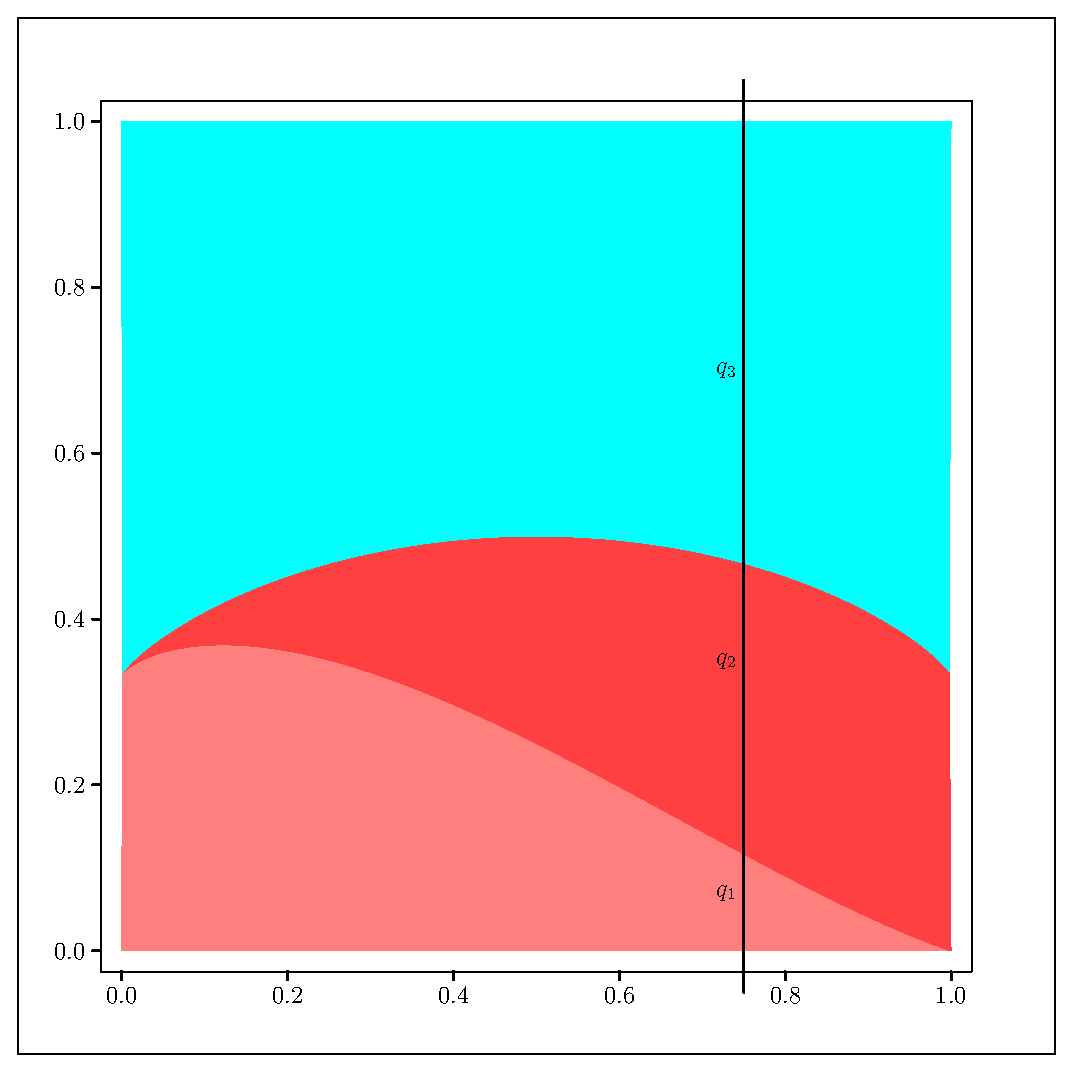
\includegraphics[width=\textwidth]{zeroone-mxnt.eps}
      \caption{Judy Benjamin's updated probability assignment using
        \textsc{maxent}. $0<{\qvu}<1$ forms the horizontal axis, the
        vertical axis shows the updated probability distribution (or
        the normalized odds vector) $(q_{1},q_{2},q_{3})$. The
        vertical line at ${\qvu}=0.75$ shows the specific updated
        probability distribution $G_{\mbox{\tiny max}}(0.75)$ for the Judy
        Benjamin problem.}
      \label{fig:mxnt}
    \end{minipage}
  \end{flushright}
\end{figure}

\section{Epistemic Entrenchment}
\label{epent}

Consider two future events $A$ and $B$. You have partial belief in
whether they will occur and assign probabilities to them. Then you
learn that $A$ entails $B$. How does this information affect your
probability assignment for event $A$? If $A$ is causally independent
of $B$ then your updated probability for it should equal the original
probability. For example, whether Sarah and Marian have sundowners at
the Westcliff hotel tomorrow may initially not depend on the weather
at all, but if they learn that there will be a wedding and the hotel's
indoor facilities will be closed to the public, then rainfall tomorrow
implies no sundowners. Learning this conditional does not affect the
probability of the antecedent (rainfall tomorrow), because the
antecedent is causally independent of the consequent.

Here is another example (the two examples are from
\scite{7}{douvenromeijn09}{}). A jeweler has been robbed, and Kate has
  reason to assume that Henry might be the robber. Kate knows that he
  is not capable of actually injuring another person, but he may very
  well engage in robbery. When Kate hears from the investigator that
  the robber also shot the jeweler she concludes that Henry is not the
  robber. She has learned a conditional and adjusted the probability
  for the antecedent. The reason for this is that Kate was
  epistemically entrenched to uphold her belief in Henry's nonviolent
  nature. Updating probabilities upon learning a conditional depends
  on epistemic entrenchments.

In Judy Benjamin's case, (HDQ) is also a conditional. If Judy is in
Red territory, she is more likely to be in the Headquarters area.
According to \textsc{maxent}, the updated probability for the
antecedent of this conditional is raised. It appears that
\textsc{maxent} preempts our epistemic entrenchments and nolens volens
assigns a certain degree of confirmation to the antecedent of a
learned conditional. This degree of confirmation depends on the causal
dependency of the antecedent on the consequent. The compatibility of
epistemic entrenchments and \textsc{maxent} is material for another
paper, but in this section we will focus on the independence
assumptions that are improperly imported into the Judy Benjamin case
by detractors of \textsc{maxent}. We will be particularly critical of
Douven and Romeijn, who hold that the Judy Benjamin case is a case for
Adam's conditioning, where the antecedent is left alone in the
updating of probabilities. 

Even though T1 is an understandably strong intuition, it does
not take into account that the information given to Judy by her
commanders may indeed be dependent on whether she is in Blue or in Red
territory. To underline this objection to intuition T1 consider three
scenarios, any of which may form the basis of the partial information
provided by her commanders.

\begin{enumerate}
\item[\textbf{I}] Judy is dropped off by a pilot who flips two
  coins. If the first coin lands H, then Judy is dropped off in Blue
  territory, otherwise in Red territory. If the second coin lands H,
  she is dropped off in the Headquarters area, otherwise in the
  Second Company area. Judy's commanders find out that the second coin
  is biased ${\qvu}:1-{\qvu}$ toward H with ${\qvu}=0.75$. The normalized odds
  vector is $G_{\mbox{\tiny I}}(0.75)=(0.125,0.375,0.500)$ and agrees
  with T1, because the choice of Blue or Red is completely independent
  from the choice of the Red Headquarters area or the Red Second
  Company area.
\item[\textbf{II}] The pilot randomly lands in any of the four
  quadrants and rolls a die. If she rolls an even number, she drops
  off Judy. If not, she takes her to another (or the same, the choice
  happens with replacement) randomly selected quadrant to repeat the
  procedure. Judy's commanders find out, however, that for $A_{1}$,
  the pilot requires a six to drop off Judy, not just an even number.
  The normalized odds vector in this scenario is $G_{\mbox{\tiny
      II}}(0.75)=(0.1,0.3,0.6)$ and does not accord with T1.
\item[\textbf{III}] Judy's commanders have divided the map into $24$
  congruent rectangles, $A_{3}$ into twelve, and $A_{1}$ and $A_{2}$
  into six rectangles each (see figures~\ref{fig:pwstex1} and
  \ref{fig:pwstex2}). They have information that the only subsets of
  the $24$ rectangles in which Judy Benjamin may be located are such
  that they contain three times as many $A_{2}$ rectangles than
  $A_{1}$ rectangles. The normalized odds vector in this scenario is
  $G_{\mbox{\tiny III}}(0.75)\approx(.108,.324,.568)$ (evaluating almost
  17 million subsets).
\end{enumerate}

I--III demonstrate the contrast between scenarios when independence is
true and when it is not. Douven and Romeijn's capital mistake in their
paper is that they assume that the Judy Benjamin problem is analogous
to their example of Sarah and sundowners at the Westcliff (see
\scite{8}{douvenromeijn09}{7}). Sarah, however, knows that whether it
rains or not is independent of her activity the next night, whereas in
Judy Benjamin we have no evidence of such independence, as scenario II
makes clear. This is not to say that scenario II is the scenario that
pertains in Judy Benjamin's case. It only says that there is no
natural assumption in Judy Benjamin's case that the probabilities are
independent of each other in light of the new evidence, for scenario
II is perfectly natural (whether it is true or not is a completely
different question) and reveals how dependence is consistent with the
information that Judy Benjamin receives.

Douven and Romeijn's strong independence claim relying on intuition T1
leads them to apply Jeffrey's rule to the Judy Benjamin problem with
the additional constraint $q_{3}=p_{3}$. They claim that in most cases
\qeins{the learning of a conditional is or would be irrelevant to
  one's degree of belief for the conditional's antecedent {\ldots} the
  learning of the relevant conditional should intuitively leave the
  probability of the antecedent unaltered}
\scite{2}{douvenromeijn09}{9}.

This, according to Douven and Romeijn, is the usual epistemic
entrenchment and applies in full force to the Judy Benjamin problem.
They give an example where the epistemic entrenchment could go the
other way and leave the consequent rather than the antecedent
unaltered (Kate and Henry, see \scite{8}{douvenromeijn09}{13}). The
idea of epistemic entrenchment is at odds with \textsc{maxent} and
seems to imply just what the full employment theorem claims: judgments
so framed \qeins{will depend on the judgmental skills of the agent,
  typically acquired not in the inductive logic class but by subject
  specific training} \scite{2}{bradley05}{349}. To pursue the
relation between the semantics of conditionals, \textsc{maxent}, and
the full employment theorem would take us too far afield at present
and shall be undertaken elsewhere. For the Judy Benjamin problem, it
is not clear why Douven and Romeijn think that the way the problem is
posed implies a strong epistemic entrenchment for Adams conditioning
(Adams conditioning is the kind of conditioning that will leave the
antecedent alone). Scenarios II-III provide realistic alternatives
where Adams conditioning is inappropriate.

Judy Benjamin may also receive ({\ref{eq:hdq}}) because her informers
have found out that Red Headquarters troops have occupied the entire
Blue territory ($q_{1}=3p_{1},q_{2}=p_{2},q_{3}=0$, the epistemic
entrenchment is with respect to $q_{2}$); because they have found out
that Blue troops have occupied two-thirds of the Red Second Company
area ($q_{1}=p_{1},q_{2}=(1/3)p_{2},q_{3}=(4/3)p_{3}$, the epistemic
entrenchment is with respect to $q_{1}$); or because they have found
out that Red Headquarters troops have taken over half of the Red
Second Company area ($q_{1}=(1/2)p_{1},q_{2}=(3/2)p_{2},q_{3}=p_{3}$,
the epistemic entrenchment is with respect to $q_{3}$ and what Douven
and Romeijn take to be an assumption in the wording of the problem).
There is nothing in the problem that supports Douven and Romeijn's
narrowing of the options. The table reiterates these options, with the
third, shaded line representing intuition (T1) and the epistemic
entrenchment defended by Douven and Romeijn.

\rowcolors{4}{lightgray}{lightgray}
\begin{tabular}{|l|c|c|c|}\hline
Epistemic entrenchment & $q_{1}$ & $q_{2}$ & $q_{3}$ \\ \hline
with respect to $A_{1}$ & 1/4 & 3/4 & 0 \\ \hline
with respect to $A_{2}$ & 1/12 & 1/4 & 2/3 \\ \hline
with respect to $A_{3}$ & 1/8 & 3/8 & 1/2 \\ \hline
\end{tabular}

\section{Coarsening at Random}

Another at first blush forceful argument that \textsc{maxent}'s
solution for the Judy Benjamin problem is counterintuitive has to do
with coarsening at random, or CAR for short. CAR involves using more
naive (or coarse) event spaces in order to arrive at solutions to
probability updating problems. The mechanics are spelled out in
\scite{1}{gruenwaldhalpern03}{}\nonsc{}. Gr{\"u}nwald and Halpern see
a parallel between the Judy Benjamin problem and Martin Gardner's
Three Prisoners problem (see \scite{8}{gardner59}{180f}). In the Three
Prisoners problem, three men (A, B, and C) are under sentence of death
when the governor decides to pardon one of them. The warden of the
prison knows which of the three men is pardoned, but none of the men
do. In a private conversation, A says to the warden, Tell me the name
of one of the others who will be executed---it will not give anything
away whether I will be executed or not. The warden agrees and tells A
that B will be executed. For the puzzling consequences, see the wealth
of literature on the Three Prisoners problem or the Monty Hall
problem.

According to Gr{\"u}nwald and Halpern, for problems of this kind (Judy
Benjamin, Three Prisoners, Monty Hall) there are naive and
sophisticated spaces to which we can apply probability updates. If A
uses the naive space, for example, he comes to the following
conclusion: of the three possibilities that (A,B), (A,C), or (B,C) are
executed, the warden's information excludes (A,C). (A,B) and (B,C) are
left over, and because A has no information about which one of these
is true his chance of not being executed is 0.5. His chance of
survival has increased from one third to one half. 

Gr{\"u}nwald and Halpern show, correctly, that the application of the
naive space is illegitimate because the CAR condition does not hold.
More generally, Gr{\"u}nwald and Halpern show that updating on the
naive space rather than the sophisticated space is legitimate for
event type observations always when the set of observations is
pairwise disjoint or, when the events are arbitrary, only when the CAR
condition holds. For Jeffrey type observations, there is a generalized
CAR condition which applies likewise. For affine constraints on which
we cannot use Jeffrey conditioning (or, a fortiori, standard
conditioning) \textsc{maxent }\qeins{essentially never gives the right
  results} \scite{2}{gruenwaldhalpern03}{243}.

Gr{\"u}nwald and Halpern conclude that \qeins{working with the naive
  space, while an attractive approach, is likely to give highly
  misleading answers} (246), especially in the application of
\textsc{maxent} to naive spaces as in the Judy Benjamin case
\qeins{where applying [\textsc{maxent}] leads to paradoxical, highly
  counterintuitive results} (245). For the Three Prisoners problem,
Jaynes' constraint rule would supposedly proceed as follows: the
vector of prior probabilities for (A,B), (A,C), and (B,C) is
$(1/3,1/3,1/3)$. The constraint is that the probability of (A,C) is
zero, and a simple application of the constraint rule yields
$(1/2,0,1/2)$ for the vector of updated probabilities. The CAR
condition for the naive space does not hold, therefore the result is
misleading.

By analogy, using the constraint rule on the naive space for the Judy
Benjamin problem yields $(0.117,0.350,0.533)$, but as the CAR
condition fails in even the simplest settings for affine constraints
(\qeins{CAR is (roughly speaking) guaranteed \emph{not} to hold except
  in \qzwei{degenerate} situations} (251), emphasis in the original),
it certainly fails for the Judy Benjamin problem, for which
constructing a sophisticated space is complicated (see
\scite{7}{grovehalpern97}{}, where the authors attempt such a
construction by retrospective conditioning).

The analogy, however, is misguided. The constraint rule has been
formally shown to generalize Jeffrey conditioning, which in turn has
been shown to generalize standard conditioning (the authors admit as
much in \scite{8}{gruenwaldhalpern03}{262}). We can solve both the
Monty Hall problem and the Three Prisoners problem by standard
conditioning, not using the naive space, but simply using the correct
space for the probability update. For the Three Prisoners problem, for
example, the warden will say either \qnull{B} or \qnull{C} in response
to A's inquiry. Because A has no information that would privilege
either answer the probability that the warden says \qnull{B} and the
probability that the warden says \qnull{C} equal each other and
therefore equal 0.5. Here is the difference between using the naive
space and using the correct space, but either way using standard
conditional probabilities:
%  ($P'$ is the prior
% probability, before A receives the warden's information, $P''$ is the
% updated probability):

\begin{displaymath}
  P(\mbox{`A is pardoned'}|\mbox{`B will be
    executed'})=
\end{displaymath}
\begin{displaymath}
  \frac{P(\mbox{`A is pardoned'})}{P(\mbox{`A is
      pardoned'})+P(\mbox{`C is pardoned'})}=\frac{1}{2}\mbox{ (incorrect)}
\end{displaymath}

\begin{displaymath}
  P(\mbox{`A is pardoned'}|\mbox{`warden says B will be
    executed'})=
\end{displaymath}
\begin{displaymath}
  \frac{P(\mbox{`A is pardoned' and `warden says B will
      be executed'})}{P(\mbox{`warden says B will be
      executed'})}=\frac{1/6}{1/2}=\frac{1}{3}\mbox{ (correct)}
\end{displaymath}

\nial Why is the first equation incorrect and the second one correct?
Information theory gives us the right answer: in the first equation,
we are conditioning on a watered down version of the evidence (watered
down in a way that distorts the probabilities because we are not
\qnull{coarsening at random}). \qnull{Warden says B will be executed}
is sufficient but not necessary for \qnull{B will be executed.} The
former proposition is more informative than the latter proposition
(its probability is lower). Conditioning on the latter proposition
leaves out relevant information contained in the wording of the
problem.

Because \textsc{maxent} always agrees with standard conditioning,
\textsc{maxent} gives the correct result for the Three Prisoners
problem. For the Judy Benjamin problem, there is no defensible
sophisticated space and no watering down of the evidence in what
Gr{\"u}nwald and Halpern call the \qnull{naive} space. The analogy
between the Three Prisoners problem and the Judy Benjamin problem as
it is set up by Gr{\"u}nwald and Halpern fails because of this crucial
difference. A successful criticism would be directed at the
construction of the \qnull{naive} space: this is what we just
accomplished for the Three Prisoners problem. There is no parallel
procedure for the Judy Benjamin problem. The \qnull{naive} space is
all we have, and \textsc{maxent} is the appropriate tool to deal with
this lack of information.

\section{The Powerset Approach}
\label{powerset}

In this section, we will focus on scenario III and consider what
happens when the grain of the partition becomes finer. We call this
the powerset approach. Two remarks are in order. On the one hand, the
powerset approach has little independent appeal. The reason behind
using \textsc{maxent} is that we want our evidence to have just the
right influence on our updated probabilities, i.e.\ neither
over-inform nor under-inform. There is no corresponding reason why we
should update our probabilities using the powerset approach. On the
other hand, what the powerset approach does is lend support to another
approach. In this task, it is persuasive because it tells us what
would happen if we were to divide the event space into infinitesimally
small, uniformly weighed, and independent \qnull{atomic} bits of
information.

In the process of arriving at the formal result, the powerset approach
resembles an empirical experiment. We are making many assumptions
favouring T1, but when the result comes in it supports T2 in
astonishingly non-trivial ways. The powerset approach provides support
for \textsc{maxent} against T1 because it combines the assumptions
grounding T1 with a limit construction and still yields a solution
that closely approximates the one generated by \textsc{maxent} rather
than the one generated by T1.

On its own the powerset approach is just what Gr{\"u}nwald and Halpern
call a naive space, for which CAR does not hold. Hence the powerset
approach will not give us a precise solution for the problem, although
it may with some plausibility guide us in the right
direction---especially if despite all its independence and uniformity
assumptions it significantly disagrees with intuition T1.

Let us assume a partition of the Blue and Red territories into sets of
equal measure (this is the division into rectangles of scenario III).
({\ref{eq:map}}) dictates that the number of sets covering $A_{3}$
equals the number of sets covering $A_{1}\cup{}A_{2}$. Initially, any
subset of this partition is a candidate for Judy Benjamin to consider.
The constraint imposed by ({\ref{eq:hdq}}) is that now we only
consider subsets for which there are three times as many partition
sets (or rectangles, although we are not necessarily limiting
ourselves to rectangles) in $A_{2}$ as there are in $A_{1}$. In
figures~\ref{fig:pwstex1} and \ref{fig:pwstex2} there are diagrams of
two subsets. One of them (figure~\ref{fig:pwstex1}) is not a
candidate, the other one (figure~\ref{fig:pwstex2}) is.

\begin{figure}[h!]
  \begin{flushright}
    \begin{minipage}[h]{\lwv\linewidth}
      \includegraphics[width=\textwidth]{partition-2.eps}
      \caption{This choice of rectangles is not a candidate because
        the number of rectangles in $A_{2}$ is not a $t$-multiple of
        the number of rectangles in $A_{1}$, here with $s=2,t=3$ as in
        scenario III.}
      \label{fig:pwstex1}
    \end{minipage}
  \end{flushright}
\end{figure}

\begin{figure}[h!]
  \begin{flushright}
    \begin{minipage}[h]{\lwv\linewidth}
      \includegraphics[width=\textwidth]{partition-1.eps}
      \caption{This choice of rectangles is a candidate because the
        number of rectangles in $A_{2}$ is a $t$-multiple of the
        number of rectangles in $A_{1}$, here with $s=2,t=3$ as in
        scenario III.}
      \label{fig:pwstex2}
    \end{minipage}
  \end{flushright}
\end{figure}

Let $X$ be the random variable that corresponds to the ratio of the
number of partition elements (rectangles) that are in $A_{3}$ to the
total number of partition elements (rectangles) for a randomly chosen
candidate. We would now anticipate that the expectation of $X$ (which
we will call $EX$) gives us an indication of the updated probability
that Judy is in $A_{3}$ (so $EX\approx{}q_{3}$). The powerset approach
is often superior to the uniformity approach (Grove and Halpern use
uniformity, with all the necessary qualifications): if you have played
Monopoly, you will know that the frequencies for rolling a 2, a 7, or
a 10 with two dice tend to conform more closely to the binomial
distribution (based on a powerset approach) rather than to the uniform
distribution with $P(\mbox{rolling }i)=1/11$ for $i=2,{\ldots},12$.

Appendix ~\ref{ThePowersetApproachFormalized} provides a formula for
the powerset approach corresponding to the formula for the
\textsc{maxent} approach, giving us $q_{3}$ dependent on $t$. Notice
that this formula is for $t=2,3,4,\ldots$. For $t=1$ use the
Chu-Vandermonde identity to find that
\begin{displaymath}
  EX_{12}=(t+1)\frac{\sum_{i=1}^{s}i\binom{ts}{i}\binom{ts}{ti}}{\sum_{i=0}^{s}\binom{ts}{i}\binom{ts}{ti}}=(t+1)\frac{s}{2}  
\end{displaymath}
and consequently $EX=1/2$, as one would expect. For
$t=1/2,1/3,1/4,\ldots$ we can simply reverse the roles of $A_{1}$ and
$A_{2}$. These results give us $G_{\mbox{\tiny pws}}$ and a graph of
the normalized odds vector (see figure~\ref{fig:pwst}), a bit bumpy
around the middle because the $t$-values are discrete and farther
apart in the middle, as $t={\qvu}/(1-{\qvu})$. Comparing the graphs of
the normalized odds vector under Grove and Halpern's uniformity
approach ($G_{\mbox{\tiny ind}}$), Jaynes' \textsc{maxent} approach
($G_{\mbox{\tiny max}}$), and the powerset approach suggested in this
paper ($G_{\mbox{\tiny pws}}$), it is clear that the powerset approach
supports \textsc{maxent}.

\begin{figure}[h!]
  \begin{flushright}
    \begin{minipage}[h]{\lwv\linewidth}
      \includegraphics[width=\textwidth]{zeroone-pwst.eps}
      \caption{Judy Benjamin's updated probability assignment
        according to the powerset approach. $0<{\qvu}<1$ forms the
        horizontal axis, the vertical axis shows the updated
        probability distribution (or the normalized odds vector)
        $(q_{1},q_{2},q_{3})$. The vertical line at ${\qvu}=0.75$ shows the
        specific updated probability distribution $G_{\mbox{\tiny
            pws}}$ for the Judy Benjamin problem.}
      \label{fig:pwst}
    \end{minipage}
  \end{flushright}
\end{figure}

Going through the calculations, it seems at many places that the
powerset approach should give its support to Grove and Halpern's
uniformity approach in keeping with intuition T1. It is unexpected to
find out that in the mathematical analysis the parameters converge to
a non-trivial factor and do not tend to negative or positive infinity.
Most surprisingly, the powerset approach, prima facie unrelated to an
approach using information, supports the idea that a set of events
about which nothing is known (such as $A_{3}$) gains in probability in
the updated probability distribution compared to the set of events
about which something is known (such as $A_{1}$ and $A_{2}$), even if
it is only partial information. Unless independence is specified, as
in Sarah and sundowners at the Westcliff, the area of ignorance gains
compared to the area of knowledge.

We now have several ways to characterize Judy's updated
probabilities and updated probabilities following upon partial
information in general. Only one of them, the uniformity approach,
violates van Fraassen, Hughes, and Harman's five symmetry requirements
in \scite{1}{fraassenetal86}{} and intuition T2. The uniformity
approach, however, is the only one that satisfies intuition T1, an
intuition which most people have when they first hear the story. 

Two arguments attenuate the position of the uniformity approach in
comparison with the others. First, T1 rests on an independence
assumption which is not reflected in the problem. Although there is no
indication that what Judy's commanders tell her is in any way
dependent on her probability of being in Blue territory, it is not
excluded either (see scenarios II and III earlier in this paper).
\textsc{maxent} takes this uncertainty into consideration. Second,
when we investigate the problem using the powerset approach it turns
out that a division into equally probable, independent, and
increasingly fine bits of information supports not intuition T1 but
rather intuition T2. \textsc{maxent}, for now, is vindicated. We need
to look for full employment not by cleverly manipulating prior
probabilities, but by making fresh observations, designing better
experiments, and partitioning the theory space more finely.

\appendix

\section{Jaynes' Constraint Rule}
\label{JaynesConstraintRule}

This appendix provides a concise but comprehensive summary of
Jaynes' constraint rule not easily obtainable in the literature.
Jaynes applied it to the Brandeis Dice Problem (see
\scite{8}{jaynes89}{243}), but does not give a mathematical
justification.

Let $f$ be a probability distribution on a finite space
$x_{1},\ldots,x_{m}$ that fulfills the constraint 
\begin{equation}
  \label{eq:constraint}
\sum_{i=1}^{m}r(x_{i})f(x_{i})=\alpha
\end{equation}

An affine constraint can always be expressed by assigning a value to
the expectation of a probability distribution (see
\scite{7}{hobson71}{}). In Judy Benjamin's case, for example, let
% This is the original line and needs to be corrected (see Sudelbuch
% p. 755)
% $r(x_{1})=0, r(x_{2})=1, r(x_{3})={\qvu}\mbox{ and }\alpha={\qvu}$. Because $f$
$r(x_{1})=0, r(x_{2})=1-{\qvu}, r(x_{3})=-{\qvu}\mbox{ and }\alpha=0$. Because $f$
is a probability distribution it fulfills
\begin{equation}
  \label{eq:unity}
\sum_{i=1}^{m}f(x_{i})=1
\end{equation}

We want to maximize Shannon's entropy, given the constraints
({\ref{eq:constraint}}) and ({\ref{eq:unity}}),
\begin{equation}
  \label{eq:entropy}
-\sum_{i=1}^{m}f(x_{i})\ln(x_{i})
\end{equation}

We use Lagrange multipliers to define the functional
\begin{equation}
  \label{eq:functional}
J(f)=-\sum_{i=1}^{m}f(x_{i})\ln{}f(x_{i})+\lambda_{0}\sum_{i=1}^{m}f(x_{i})+\lambda_{1}\sum_{i=1}^{m}r(x_{i})f(x_{i})\notag
\end{equation}
and differentiate it with respect to $f(x_{i})$
\begin{equation}
  \label{eq:funder}
\frac{\partial{}J}{\partial{}f(x_{i})}=-\ln(f(x_{i}))-1+\lambda_{0}+\lambda_{1}r(x_{i})
\end{equation}

Set ({\ref{eq:funder}}) to $0$ to find the necessary condition to
maximize ({\ref{eq:entropy}})
\begin{equation}
  \label{eq:coverthomas}
g(x_{i})=e^{\lambda_{0}-1+\lambda_{1}r(x_{i})}\notag
\end{equation}

This is the Gibbs distribution. We still need to do two things: (a)
show that the entropy of $g$ is maximal, and (b) show how to find
$\lambda_{0}$ and $\lambda_{1}$. (a) is shown in Theorem 12.1.1 in
Cover and Thomas \scite{1}{coverthomas06}{} and there is no reason to
copy it here. 

For (b), let
\begin{equation}
  \label{eq:l1}
\lambda_{1}=-\beta\notag
\end{equation}
\begin{equation}
  \label{eq:zet}
Z(\beta)=\sum_{i=1}^{m}e^{-\beta{}r(x_{i})}\notag
\end{equation}
\begin{equation}
  \label{eq:l0}
\lambda_{0}=1-\ln(Z(\beta))\notag
\end{equation}

To find $\lambda_{0}$ and $\lambda_{1}$ we introduce the constraint
\begin{equation}
  \label{eq:logcon}
-\frac{\partial}{\partial{}\beta}\ln(Z(\beta))=\alpha\notag
\end{equation}

To see how this constraint gives us $\lambda_{0}$ and $\lambda_{1}$,
Jaynes' solution of the Brandeis Dice Problem (see
\scite{8}{jaynes89}{243}) is a helpful example. We are, however,
interested in a general proof that this choice of $\lambda_{0}$ and
$\lambda_{1}$ gives us the probability distribution maximizing the
entropy. That $g$ so defined maximizes the entropy is shown in (a). We
need to make sure, however, that with this choice of $\lambda_{0}$ and
$\lambda_{1}$ the constraints ({\ref{eq:constraint}}) and
({\ref{eq:unity}}) are also fulfilled.

First, we show
\begin{align}
&\sum_{i=1}^{m}g(x_{i})=\sum_{i=1}^{m}e^{\lambda_{0}-1+\lambda_{1}r(x_{i})}=e^{\lambda_{0}-1}\sum_{i=1}^{m}e^{\lambda_{1}r(x_{i})}=\notag\\
&e^{-\ln(Z(\beta))}Z(\beta)=1\label{eq:unishow}\notag
\end{align}

Then, we show, by differentiating $\ln(Z(\beta))$ using the
substitution $x=e^{-\beta}$
\begin{align}
&\alpha=-\frac{\partial}{\partial{}\beta}\ln(Z(\beta))=-\frac{1}{\sum_{i=1}^{m}x^{r(x_{i})}}\left(\sum_{i=1}^{m}r(x_{i})x^{r(x_{i})-1}\right)(-x)=\notag\\
&\frac{\sum_{i=1}^{m}r(x_{i})x^{r(x_{i})}}{\sum_{i=1}^{m}x^{r(x_{i})}}\notag
\end{align}

And, finally,
\begin{align}
&\sum_{i=1}^{m}r(x_{i})g(x_{i})=\sum_{i=1}^{m}r(x_{i})e^{\lambda_{0}-1+\lambda_{1}r(x_{1})}=e^{\lambda_{0}-1}\sum_{i=1}^{m}r(x_{i})e^{\lambda_{1}r(x_{1})}=\notag\\
&e^{\lambda_{0}-1}\sum_{i=1}^{m}r(x_{i})x^{r(x_{i})}=\alpha{}e^{\lambda_{0}-1}\sum_{i=1}^{m}x^{r(x_{i})}=\alpha{}e^{\lambda_{0}-1}\sum_{i=1}^{m}e^{-\beta{}r(x_{i})}=\notag\\
&\alpha{}Z(\beta)e^{\lambda_{0}-1}=\alpha{}Z(\beta))e^{-\ln(Z(\beta))}=\alpha\notag
\end{align}

Filling in the variables from Judy Benjamin's scenario gives us result
({\ref{eq:vmax}}). The lambdas are:
  \begin{displaymath}
    \lambda_{0}=1-\ln\left(\sum_{i=1}^{m}e^{\lambda_{1}r(x_{i})}\right)\hspace{.3in}
    \lambda_{1}=\ln{}{\qvu}-\ln(1-{\qvu})\notag
  \end{displaymath}

  We combine the normalized odds vector $(0.16,0.48,0.36)$ following
  from these lambdas using Dempster's Rule of Combination with
  ({\ref{eq:map}}) and get result ({\ref{eq:vmax}}).

\section{The Powerset Approach Formalized}
\label{ThePowersetApproachFormalized}

Let us assume a partition $\{B_{i}\}_{i=1,{\ldots},4n}$ of
$A_{1}\cup{}A_{2}\cup{}A_{3}$ into sets that are of equal measure
$\mu$ and whose intersection with $A_{i}$ is either the empty set or
the whole set itself (this is the division into rectangles of scenario
III). ({\ref{eq:map}}) dictates that the number of sets covering
$A_{3}$ equals the number of sets covering $A_{1}\cup{}A_{2}$. For
convenience, we assume the number of sets covering $A_{1}$ to be $n$.
Let $\mathcal{C}$, a subset of the powerset of
$\{B_{i}\}_{i=1,{\ldots},4n}$, be the collection of sets which agree
with the constraint imposed by ({\ref{eq:hdq}}), i.e.\
\begin{displaymath}
  C\in\mathcal{C}\mbox{ iff }C=\{C_{j}\}\mbox{ and }t\mu\left(\bigcup{}C_{j}\cap{}A_{1}\right)=\mu\left(\bigcup{}C_{j}\cap{}A_{2}\right)
\end{displaymath}
In figures~\ref{fig:pwstex1} and \ref{fig:pwstex2} there are diagrams
of two elements of the powerset of $\{B_{i}\}_{i=1,{\ldots},4n}$. One
of them (figure~\ref{fig:pwstex1}) is not a member of $\mathcal{C}$,
the other one (figure~\ref{fig:pwstex2}) is.

The binomial distribution dictates the expectation $EX$ of $X$, using
simple combinatorics. In this case we require, again for convenience,
that $n$ be divisible by $t$ and the \qnull{grain} of the partition
$A$ be $s=n/t$. Remember that $t$ is the factor by which
({\ref{eq:hdq}}) indicates that Judy's chance of being in $A_{2}$ is
greater than being in $A_{1}$. In Judy's particular case, $t=3$ and
${\qvu}=0.75$. We introduce a few variables which later on will help
for abbreviation:
\begin{displaymath}
n=ts\hspace{.5in}
2m=n\hspace{.5in}
2j=n-1\hspace{.5in}
{T}=t^{2}+1
\end{displaymath}
$EX$, of course, depends both on the grain of $A$ and the value of
$t$. It makes sense to make it independent of the grain by letting the
grain become increasingly finer and by determining $EX$ as
$s\rightarrow\infty$. This cannot be done for the binomial
distribution, as it is notoriously uncomputable for large numbers
(even with a powerful computer things get dicey around $s=10$). But,
equally notorious, the normal distribution provides a good
approximation of the binomial distribution and will help us arrive at
a formula for $G_{\mbox{\tiny pws}}$ (corresponding to 
$G_{\mbox{\tiny ind}}$ and $G_{\mbox{\tiny max}}$), determining the value $q_{3}$
dependent on ${\qvu}$ as suggested by the powerset approach.

First, we express the random variable $X$ by the two independent
random variables $X_{12}$ and $X_{3}$. $X_{12}$ is the number of
partition elements in the randomly chosen $C$ which are either in
$A_{1}$ or in $A_{2}$ (the random variable of the number of partition
elements in $A_{1}$ and the random variable of the number of partition
elements in $A_{2}$ are decisively not independent, because they need
to obey ({\ref{eq:hdq}})); $X_{3}$ is the number of partition elements
in the randomly chosen $C$ which are in $A_{3}$. A relatively simple
calculation shows that $EX_{3}=n$, which is just what we would expect
(either the powerset approach or the uniformity approach would give us
this result):
\begin{displaymath}
  EX_{3}=2^{-2n}\sum_{i=0}^{2n}i\binom{2n}{i}=n\mbox{ (use }\binom{n}{k}=\frac{n}{k}\binom{n-1}{k-1}\mbox{)}
\end{displaymath}

The expectation of $X$, $X$ being the random variable expressing the
ratio of the number of sets covering $A_{3}$ and the number of sets
covering $A_{1}\cup{}A_{2}\cup{}A_{3}$, is
\begin{displaymath}
  EX=\frac{EX_{3}}{EX_{12}+EX_{3}}=\frac{n}{EX_{12}+n}
\end{displaymath}
If we were able to use uniformity and independence, $EX_{12}=n$ and
$EX=1/2$, just as Grove and Halpern suggest (although their uniformity
approach is admittedly less crude than the one used here). Will the
powerset approach concur with the uniformity approach, will it support
the principle of maximum entropy, or will it make another suggestion
on how to update the prior probabilities? To answer this question, we
must find out what $EX_{12}$ is, for a given value $t$ and
$s\rightarrow\infty$, using the binomial distribution and its
approximation by the normal distribution.

Using combinatorics,
\begin{displaymath}
  EX_{12}=(t+1)\frac{\sum_{i=1}^{s}i\binom{ts}{i}\binom{ts}{ti}}{\sum_{i=0}^{s}\binom{ts}{i}\binom{ts}{ti}}
\end{displaymath}

Let us call the numerator of this fraction NUM and the denominator
DEN. According to the de Moivre-Laplace Theorem,
\begin{displaymath}
  \mbox{DEN}=\sum_{i=0}^{s}\binom{ts}{i}\binom{ts}{ti}\approx{}2^{2n}\sum_{i=0}^{s}\int_{i-\frac{1}{2}}^{i+\frac{1}{2}}\mathcal{N}(\frac{n}{2},\frac{n}{4})(i)\mathcal{N}(\frac{n}{2},\frac{n}{4})(ti)di
\end{displaymath}
where
\begin{displaymath}
  \mathcal{N}(\mu,\sigma^{2})(x)=\frac{1}{\sqrt{2\pi\sigma^{2}}}\exp\left(-\frac{(x-\mu)^{2}}{2\sigma^{2}}\right)
\end{displaymath}
Substitution yields
\begin{displaymath}
  \mbox{DEN}\approx{}2^{2n}\frac{1}{\pi{}m}\sum_{i=0}^{s}\int_{i-\frac{1}{2}}^{i+\frac{1}{2}}\exp\left(-\frac{\left(x-m\right)^{2}}{m}-\frac{t^{2}\left(x-\frac{m}{t}\right)^{2}}{m}\right)dx
\end{displaymath}
Consider briefly the argument of the exponential function:
\begin{displaymath}
  -\frac{\left(x-m\right)^{2}}{m}-\frac{t^{2}\left(x-\frac{m}{t}\right)^{2}}{m}=-\frac{t^{2}}{m}({\aden}x^{2}+{\bden}x+{\cden})=-\frac{t^{2}}{m}\left({\aden}(x-{\hden})^{2}+{\kden}\right)
\end{displaymath}
with (the double prime sign corresponds to the simple prime sign for
the numerator later on)
\begin{displaymath}
{\aden}=\frac{1}{t^{2}}{T}\notag\hspace{.5in}
{\bden}=(-2m)\frac{1}{t^{2}}(t+1)\hspace{.5in}
{\cden}=2m^{2}\frac{1}{t^{2}}
\end{displaymath}
\begin{displaymath}
{\hden}=-{\bden}/2{\aden}\hspace{.5in}
{\kden}={\aden}{\hden}^{2}+{\bden}{\hden}+{\cden}
\end{displaymath}
Consequently,
\begin{displaymath}
\mbox{DEN}\approx{}2^{2n}\exp\left(-\frac{t^{2}}{m}{\kden}\right)\sqrt{\frac{1}{\pi{}{\aden}mt^{2}}}\int_{-\infty}^{s+\frac{1}{2}}\mathcal{N}\left({\hden},\frac{m}{2{\aden}t^{2}}\right)dx
\end{displaymath}
And, using the error function for the cumulative density function of
the normal distribution,
\begin{equation}
  \label{eq:den}
  \mbox{DEN}\approx{}2^{2n-1}\sqrt{\frac{1}{\pi{}{\aden}mt^{2}}}\exp\left(-\frac{{\kden}t^{2}}{m}\right)\left(1-\erf({\wden})\right)
\end{equation}
with
\begin{displaymath}
  {\wden}=\frac{t\sqrt{{\aden}}\left(s+\frac{1}{2}-{\hden}\right)}{\sqrt{m}}
\end{displaymath}

We proceed likewise with the numerator, although the additional factor
introduces a small complication:
  \begin{eqnarray*}
  \mbox{NUM}&=&\sum_{i=1}^{s}i\binom{ts}{i}\binom{ts}{ti}=\sum_{i=1}^{s}s\binom{ts}{i}\binom{ts-1}{ti-1}\\
&\approx&s2^{2n-1}\sum_{i=1}^{s}\mathcal{N}\left(m,\frac{m}{2}\right)(i)\mathcal{N}\left(j,\frac{j}{2}\right)(ti-1)
\end{eqnarray*}
Again, we substitute and get
\begin{displaymath}
  \mbox{NUM}\approx{}s2^{2n-1}\left(\pi\sqrt{mj}\right)^{-1}\sum_{0}^{s-1}\int_{i-\frac{1}{2}}^{i+\frac{1}{2}}\exp\left({\anum}(x-{\hnum})^{2}+{\knum}\right)
\end{displaymath}
where the argument for the exponential function is
\begin{displaymath}
  -\frac{1}{mj}\left(j(x-m)^{2}+mt^{2}\left(x-\frac{j+1}{t}\right)^{2}\right)
\end{displaymath}
and therefore
\begin{displaymath}
{\anum}=j+mt^{2}\hspace{.5in}
{\bnum}=2j(1-m)+2mt\left(t-j\right)\hspace{.5in}
{\cnum}=j(1-m)^{2}+m\left(t-j-1\right)^{2}
\end{displaymath}
\begin{displaymath}
{\hnum}=-{\bnum}/2{\anum}\hspace{.5in}
{\knum}={\anum}{\hnum}^{2}+{\bnum}{\hnum}+{\cnum}
\end{displaymath}
Using the error function, 
\begin{equation}
  \label{eq:num}
  \mbox{NUM}\approx{}2^{2n-2}\frac{s}{\sqrt{\pi{}{\anum}}}\exp\left(-\frac{{\knum}}{mj}\right)\left(1+\erf({\wnum})\right)
\end{equation}
with
\begin{displaymath}
  {\wnum}=\frac{\sqrt{{\anum}}\left(s-\frac{1}{2}-{\hnum}\right)}{\sqrt{mj}}
\end{displaymath}

Combining ({\ref{eq:den}}) and ({\ref{eq:num}}),
\begin{eqnarray*}
  EX_{12}&=&(t+1)\frac{\mbox{NUM}}{\mbox{DEN}}\\
&\approx&\frac{1}{2}(t+1)\sqrt{\frac{{T}{}ts}{{T}{}ts-1}}se^{\alpha_{t,s}}
\end{eqnarray*}
for large $s$, because the arguments for the error function $w'$ and
$w''$ escape to positive infinity in both cases (NUM and DEN) so that
their ratio goes to 1. The argument for the exponential function is
\begin{displaymath}
  \alpha_{t,s}=-\frac{{\knum}}{mj}+\frac{{\kden}t^{2}}{m}
\end{displaymath}
and, for $s\rightarrow\infty$, goes to
\begin{displaymath}
  \alpha_{t}=\frac{1}{2}{T}^{-2}(2t^{3}-3t^{2}+4t-5)
\end{displaymath}

Notice that, for $t\rightarrow\infty$, $\alpha_{t}$ goes to $0$ and
\begin{displaymath}
  EX=\frac{n}{EX_{12}+n}\rightarrow\frac{2}{3}
\end{displaymath}
in accordance with intuition T2.

% BibTeX users please use one of
% \bibliographystyle{stefan-2010-08-28} 
\bibliographystyle{spbasic}      % basic style, author-year citations
%\bibliographystyle{spmpsci}      % mathematics and physical sciences
%\bibliographystyle{spphys}       % APS-like style for physics
%\bibliography{}   % name your BibTeX data base
\bibliography{bib-3306}

% % Non-BibTeX users please use
% \begin{thebibliography}{}
% %
% % and use \bibitem to create references. Consult the Instructions
% % for authors for reference list style.
% %
% \bibitem{RefJ}
% % Format for Journal Reference
% Author, Article title, Journal, Volume, page numbers (year)
% % Format for books
% \bibitem{RefB}
% Author, Book title, page numbers. Publisher, place (year)
% % etc
% \end{thebibliography}

\end{document}
% end of file template.tex
